\documentclass[12pt,a4paper]{article}
%\documentclass[11pt,UTF8]{article}
%\usepackage{ctex}
\usepackage{tcolorbox}
\usepackage{graphicx}
\usepackage{geometry}
\usepackage{listings}
\usepackage{xcolor}
\usepackage{mathtools}
\usepackage{framed} 
\usepackage{amsfonts}
\usepackage{algpseudocode} 
\usepackage{algorithm}
\usepackage{ulem}
\usepackage{tikz}

\renewcommand{\algorithmicrequire}{ \textbf{Input:}} %Use https://www.overleaf.com/project/6038f72fd2827e6248936428Input in the format of Algorithm
\renewcommand{\algorithmicensure}{ \textbf{Output:}} %Use Output in the format of Algorithm
\definecolor{codegreen}{rgb}{0,0.6,0}
\definecolor{codegray}{rgb}{0.5,0.5,0.5}
\definecolor{codepurple}{rgb}{0.58,0,0.82}
\definecolor{backcolour}{rgb}{0.95,0.95,0.92}

\usepackage{tikz}
\usepackage{tikz-qtree}

\begin{document}
\noindent

%========================================================================
\noindent\framebox[\linewidth]{\shortstack[c]{
\Large{\textbf{Homework 6}}\vspace{1mm}\\
VE216 - Introduction to Signal and Systems, Qiao Heng, Spring 2021}}

\begin{center}

\footnotesize{\color{blue}$*$ Name: Han Yibei \quad\quad\quad\quad\quad\quad Student ID: 519370910123}
\end{center}

\section*{HW Notes:}
\begin{itemize}
    \item Problems where the number of points are followed by an exclamation are basic skill problems and will be graded without partial credit.
    \item \fbox{Box} your final answer. You will be graded on both the final answer and the steps leading to it. Correct intermediate steps will help earn partial credit.
    For full credit, \sout{cross out} any incorrect intermediate step.
    \item If you need to make any additional assumptions, state them clearly.
    \item Legible writing will help when it comes to partial credit.
    \item Simplify your result when possible.
\end{itemize}

\section*{Problems:}
\normalsize
\begin{tcolorbox}[colback = white]
1. [5] Is this system stable? Explain. (Note: the system is causal.)\\
$$
2 \cdot 10^{6} y(t)+10^{5} \frac{d}{d t} y(t)+60 \frac{d^{2}}{d t^{2}} y(t)+\frac{d^{3}}{d t^{3}} y(t)=8 \cdot 10^{6} x(t)-10^{4} \frac{d}{d t} x(t)
$$

\end{tcolorbox}

\begin{tcolorbox}
\normalsize
\textcolor{blue}{Answer:\\
$$y(t)(2\times 10^6+10^5 s+60 s^2+s^3)=x(t)(8\times 10^6-10^4 s)$$
$$\frac{y(t)}{x(t)}=\frac{8\times 10^6-10^4 s}{2\times 10^6+10^5 s+60 s^2+s^3}$$
$$\text{Let } 2\times 10^6+10^5 s+60 s^2+s^3=0 \text{ we can get } s_1=20.16~~s_{2,3}=-19.9\pm 314.3j$$
The poles are all in the LHS and the ROC contains the $j\omega$ axis, so it is \fbox{stable}
}
\end{tcolorbox}

\begin{tcolorbox}[colback = white]
2. [10] A unit step signal is applied to a system consisting of two LTI system connected in parallel. The pole-zero plots of each of the system are shown below. Determine the output signal. Assume that each of
the system has unit gain at DC.
\begin{figure}[H]
	\centering
	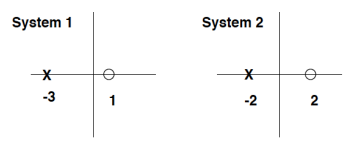
\includegraphics{HW6P2.png}
	\label{fig:fig1} 
\end{figure}
Hint:first find the Laplace transform $Y(s)$ of the output signal using the convolution and linearity properties of the Laplace transform, Then take the inverse Laplace transform to get $y(t)$ using PFE. The “unit gain at DC” specifies $H_{1}(0)$ and $H_{2}(0)$, which you can use to determine the scaling factor.

\end{tcolorbox}

\begin{tcolorbox}
\normalsize
\textcolor{blue}{Answer:\\
$$H_1(s)=G_1\times\frac{s-1}{s+3}~~~~Y_2(s)=G_2\times\frac{s-2}{s+2}$$
$$G=\frac{b_m}{a_0}~~1=G_1\times-\frac{1}{3}~~1=G_2\times -1$$
\begin{equation*}
    \begin{aligned}
        Y(s)&=X(s)(H_1(s)+H_2(s))=X(s)(\frac{3-3s}{3+s}+\frac{2-s}{2+s})\\
        &=-\frac{1}{s}\frac{4(s^2+s-3)}{(s+2)(s+3)}=\frac{2}{s}-\frac{4}{s+3}-\frac{2}{s+2}
    \end{aligned}
\end{equation*}
$Real\{s\}>0$ and $y(t)=2u(t)-4e^{-3t}u(t)-2e^{-2t}u(t)$
}
\end{tcolorbox}

\begin{tcolorbox}[colback = white]
3. [20] Consider an LTI system with input $x(t)=e^{-t}u(t)$ and impulse response $h(t)=e^{-2t}u(t)$. \\
(a) Determinse the Laplace transform of $x(t)$ and $h(t)$.\\
(b) Using the convolution property, determine the Laplace transform $Y(s)$ of the output $y(t)$.\\
(c) From the Laplace transform of $y(t)$ as obtained in part(b), determine $y(t)$.\\
(d) Verify your result in part (c) by explicitly convolving $x(t)$ and $h(t)$.\\


\end{tcolorbox}

\begin{tcolorbox}
\normalsize
\textcolor{blue}{Answer:\\
(a) $x(t)\stackrel{\mathcal{L}}{\longleftrightarrow}\frac{1}{s+1}~~~~h(t)\stackrel{\mathcal{L}}{\longleftrightarrow}\frac{1}{s+2}$\\
(b) $Y(s)=X(s)\cdot H(s)=\frac{1}{(s+2)(s+1)}$\\
(c) $\frac{1}{(s+2)(s+3)}=\frac{1}{s+1}-\frac{1}{s+2}$\\
$\Rightarrow y(t)=e^{-t}u(t)+e^{-2t}u(t)$\\
(d) $y(t)=x(t)*h(t)=\int_{-\infty}^\infty x(t-\tau)h(\tau)d\tau=e^{-t}u(t)+e^{-2t}u(t)$
}
\end{tcolorbox}

\begin{tcolorbox}[colback = white]
4. [20] The system function of a causal LTI system is
$$
H(s)=\frac{s+1}{s^{2}+2s+2}
$$
Determine and sketch the response $y(t)$ when the input is
$$
e^{-|t|}, \quad-\infty<t<\infty
$$
\end{tcolorbox}

\begin{tcolorbox}
\normalsize
\textcolor{blue}{Answer:\\
$x(t)\stackrel{\mathcal{L}}{\longleftrightarrow}\frac{2}{1-s^2}$, then $Y(s)=X(s)\cdot H(s)=\frac{1}{(s^2+2s+2)(1-s)}$\\
$$Y(s)=\frac{2}{5}(\frac{s+1}{(s+1)^2+1})+\frac{2}{(s+1)^2+1}-\frac{1}{s-1}$$
$$y(t)=\frac{2}{5}coste^{-t}u(t)+\frac{4}{5}sinte^{-t}u(t)+\frac{2}{5}e^tu(-t)$$
\begin{figure}[H]
    \centering
    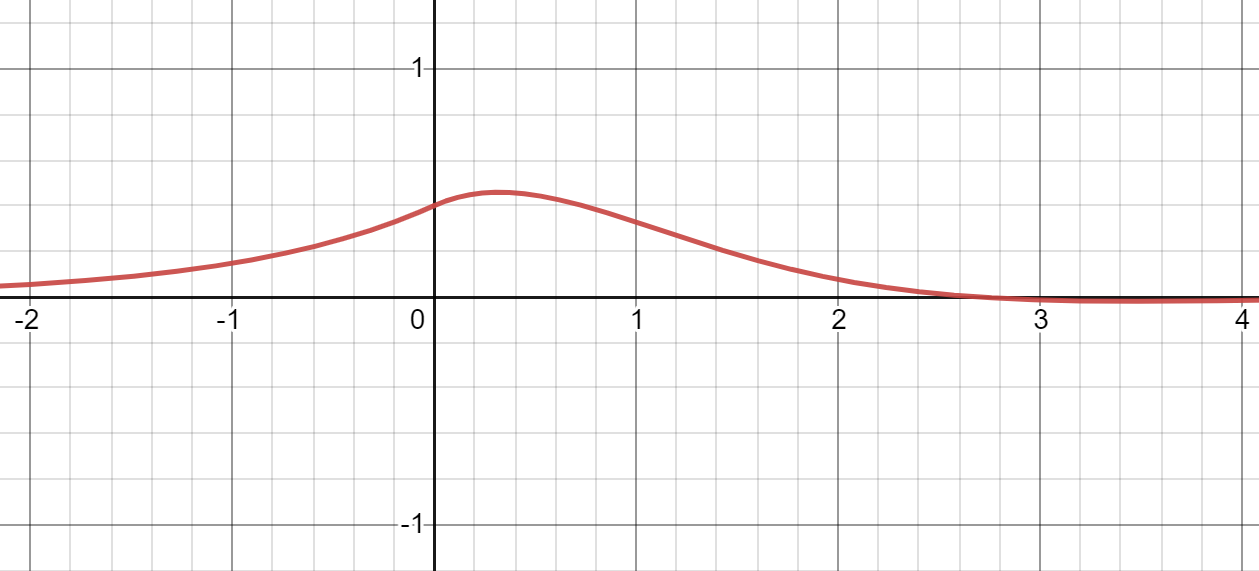
\includegraphics[width=8cm]{q4.png}
\end{figure}
}
\end{tcolorbox}

\begin{tcolorbox}[colback = white]
5. [45]  In this problem, we consider the construction of various type of block diagram representations for a
causal LTI system S with input $x(t)$, output $y(t)$, and system function
$$
H(s)=\frac{2s^{2}+4s-6}{s^{2}+3s+2}
$$
To derive the direct-diagram representation of $S$, we first consider a causal LTI system S1 that has the same input $x(t)$ as $S$, but whose system function is
$$
H(s)=\frac{1}{s^{2}+3s+2}
$$
With the output of $S_{1}$ denoted by $y_{1}(t)$, the direct-form diagram representation of $S_{1}$ is shown in Figure below. The signals $e(t)$ and $f(t)$ indicates in the figure represent respective inputs into the two integrators.\\
(a) Express $y(t)$ (the output of S) as a linear combination of $y_{1}(t)$, $\frac{dy_{1}t}{dt}$, and $\frac{d^{2}y_{1}(t)}{dt^{2}}$.\\
(b) How is $\frac{dy_{1}t}{dt}$ related to $f(t)$.\\
(c) How is $\frac{d^{2}y_{1}(t)}{dt^{2}}$ related to $e(t)$.\\
(d) Express $y(t)$ as a linear combination of $e(t)$, $f(t)$, $y_{1}(t)$.\\
(e) Use the result from the previous part to extend the direct-form block diagram representation of $S_{1}$ and create a block diagram representation of $S$.\\
(f) Observing that
$$
H(s)=\left(\frac{2(s-1)}{s+2}\right)\left(\frac{s+3}{s+1}\right)
$$
draw a block diagram representation for S as a cascade combination of two subsystems.\\
(g) Observing that
$$
H(S)=2+\frac{6}{s+2}-\frac{8}{s+1}
$$
draw a block-diagram representation for S as parallel combination of three subsystems.
\begin{figure}[H]
	\centering
	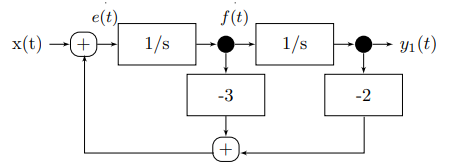
\includegraphics{HW6P5.png}
	\label{fig:fig2} 
\end{figure}
\end{tcolorbox}

\begin{tcolorbox}
\normalsize
\textcolor{blue}{Answer:\\
(a) $$y(t)=2\frac{d^2y_1t}{dt^2}+4\frac{dy_1(t)}{dt}-6y_1(t)$$
(b) $\frac{dy_1t}{dt}=f(t)$\\
(c) $\frac{d^2y_1t}{dt^2}=e(t)$\\
(d) $y(t)=2e(t)+4f(t)-6y_1(t)$
\begin{figure}[H]
    \centering
    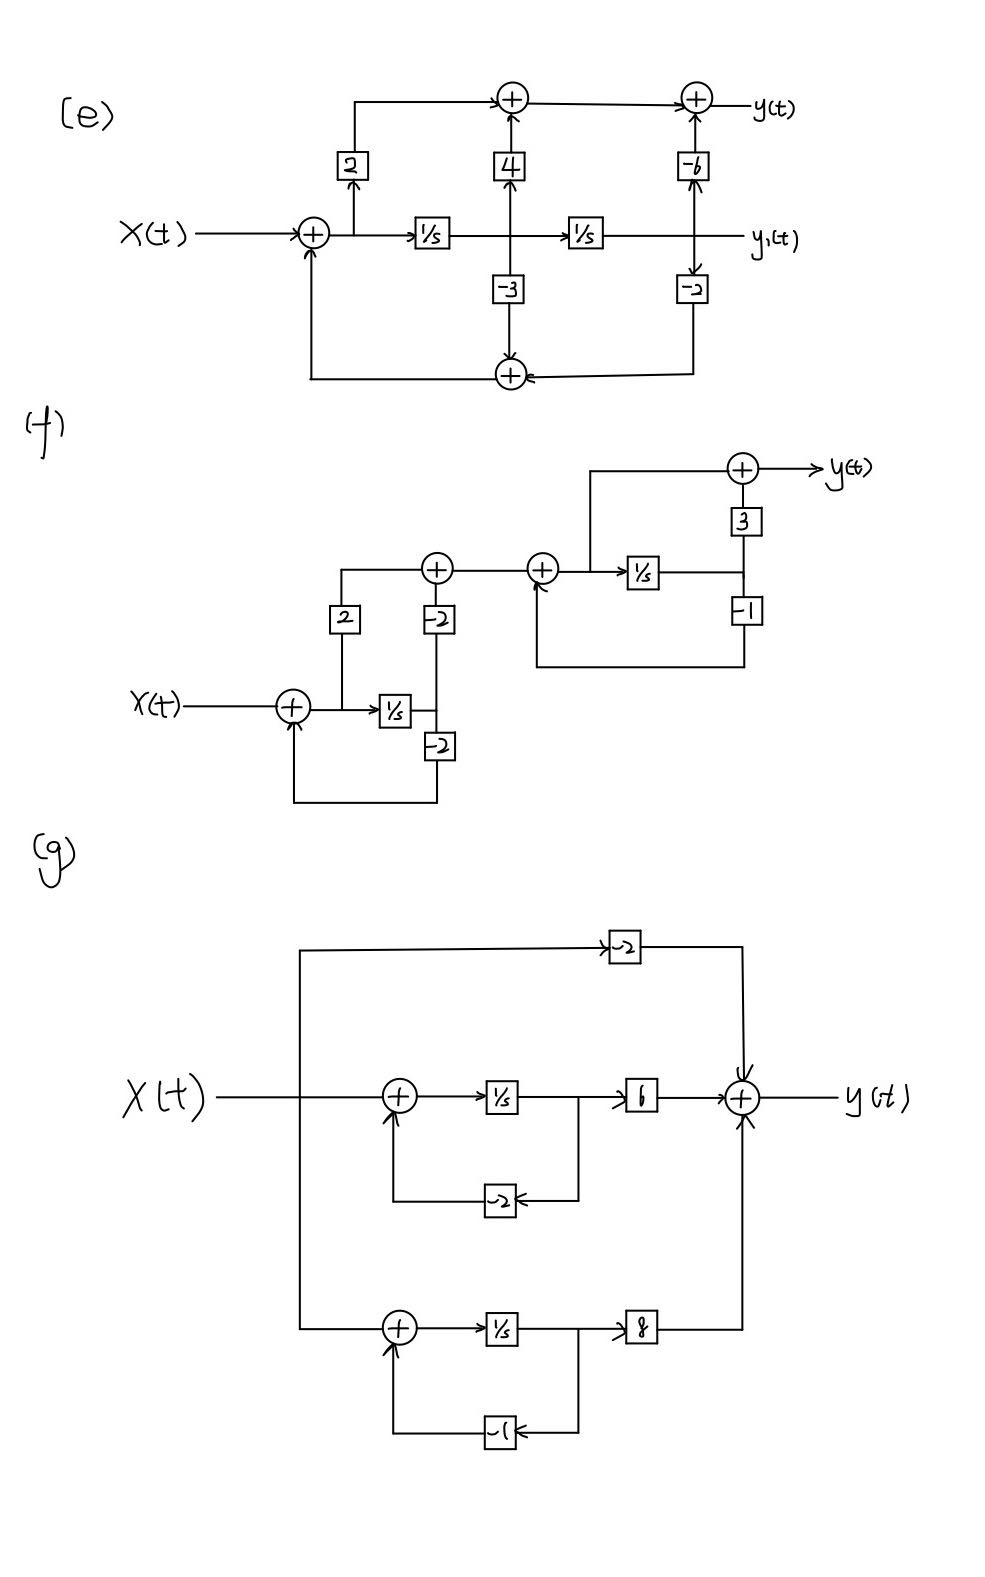
\includegraphics[width=10cm]{5.jpg}
\end{figure}
}
\end{tcolorbox}


%========================================================================
\end{document}

